\documentclass{beamer}

%% GRAPHICS
% tikz - of course
\usepackage{tikz}
\usetikzlibrary{arrows,snakes,shapes}
\usepackage{graphicx}
\setkeys{Gin}{width=\linewidth, height=0.8\textheight, keepaspectratio=true}
\usepackage[final]{movie15}
\usepackage[utf8]{inputenc}
\usetheme{WillBlack}
\definecolor[named]{meanbg}{RGB}{255,255,255} %should be mean color of bg image

\graphicspath{
  {../media/},
}

\title{Un viaje a la Nebulosa de Orión}
\author
{
  William J. Henney
}                               %

\institute[CRyA, UNAM]
{
  Centro de Radioastronomía y Astrofísica\\
  UNAM, Morelia, México
}


\begin{document}

\begin{frame}
  \titlepage
\end{frame}

\begin{frame}
  \frametitle{El sol en la Vía Láctea}
  % Note that autoresume should not be used, since it cancels autoplay
  \includemovie[label=sun-milkyway, autoplay, autopause, repeat, palindrome]
  {\textwidth}{0.5625\textwidth}{hst15_milky_way4.mp4}
\end{frame}

\begin{frame}
  \frametitle{La Gran Nebulosa de Orión}
  \includemovie[label=orion-zoom, poster, autopause]
  {\textwidth}{0.75\textwidth}{Orion-long-zoom-high_quicktime.mov}
\end{frame}

\begin{frame}
  \frametitle{El lado escondido de Orión}
  \includemovie[label=orion-nicmos, autoplay, autopause, repeat, palindrome]
  {0.8\textwidth}{0.533\textwidth}{hs-1997-13-a-low_quicktime.mov}
  \begin{block}{La luz óptica contra La luz infrarroja}
    La lus infrarroja penetra más facilmente el polvo,\\ 
    revelando las estrellas jóvenes
    atrás de la nebulosa
  \end{block}
\end{frame}

\begin{frame}
  \frametitle{Más sobre el lado escondido}
  {}\hfill
  \includegraphics<1>[height=\textheight]{orion_vis}
  \includegraphics<2>[height=\textheight]{orion_ir}
  \transsplitverticalout<2>[duration=1]
\end{frame}

\begin{frame}
  \frametitle{La nube molécular atrás de la nebulosa}
  \includegraphics<1>[height=\textheight]{LargeScale-1}
  \includegraphics<2>[height=\textheight]{LargeScale-2}
  \includegraphics<3>[height=\textheight]{LargeScale-1-2}
  \includegraphics<4>[height=\textheight]{LargeScale-1-2-3}
\end{frame}


\begin{frame} \frametitle{El corazón de la nebulosa de Orión}
  \setkeys{Gin}{width=\textwidth, height=0.8\textheight, keepaspectratio=true}
  \includegraphics<1>{All_quart}%
  \includegraphics<2>{All_quart_hilight}
  \includegraphics<3>{talk_image_658+656+502}%
  \includegraphics<4>{talk_image_658+673+631}%
\end{frame}

\tikzstyle{photonstyle}=[->, >=open triangle 45,
ultra thick,  color=blue, semitransparent, 
snake=snake, 
segment amplitude=5pt, 
segment length=15pt,
line after snake=12pt]

\newcommand\photons{%
  \draw[style=photonstyle] (-140:1.0) -- (-140:4.0);
  \draw[style=photonstyle] (-160:1.5) -- (-160:4.5);
  \draw[style=photonstyle] (-170:2.5) -- (-170:5.5);
}
\newcommand\myarrow{%
  % pinch in the upstroke
  (0, 0) .. controls +(60:0.3) and +(-60:0.3) .. ++(80:1) 
  % sweep back the head
  -- ++(200:0.2) -- ++(70:0.5) -- ++(-50:0.5) -- ++(180:0.2)
  % and curve out the downstroke
  .. controls +(-70:0.3) and +(70:0.3) .. (0.3,-0.1) -- cycle
  }

\begin{frame} \frametitle{¿Qué es un proplyd?}
  \begin{tikzpicture}
    \path[use as bounding box, draw, dashed, fill=meanbg](-1, -1) rectangle (8, 3);
    \begin{scope}[shift={(1,0.3)}, rotate=-30]
      % disk
      \shade[
      scale=1.6,
      shading=radial, inner color=green!20!black, outer color=meanbg
      ] 
      (165:1) arc (165:195:1) -- +(15:2) arc (15:-15:1) -- cycle;
      % low-mass star
      \only<2->{
        \shade[ball color=red] (0, 0) circle (.2);
      }
      \only<3->{
        \begin{scope}
          [bottom color=meanbg, 
          top color=red!50!black,
          shift={(north:0.2)}]
          \shade[shift={(-1.3,0.4)}, rotate=30] \myarrow ; 
          \shade[shift={(-0.5,0.2)}, xslant=-0.1, rotate=15, scale=1.3] \myarrow ; 
          \begin{scope}[xscale=-1]
            \shade[shift={(-1.3,0.4)}, rotate=30] \myarrow ; 
            \shade[shift={(-0.5,0.2)}, xslant=-0.1, rotate=15, scale=1.3] \myarrow ; 
          \end{scope}
        \end{scope}
      }
    \end{scope}
    \begin{scope}[shift={(6,2.3)}]
      \only<4->\photons
      \only<5>{
        \path[shade, ball color=blue!50!cyan] (0,0) circle (.4);
      }
    \end{scope}
  \end{tikzpicture}
  \bigskip
  \begin{block}{Un proplyd es \dots}
    \dots un disco circunestelar\dots\pause en torno a una estrella
    jóven de baja masa\dots\pause lo cual se está
    evaporando\dots\pause por la radiación ultravioleta\dots\pause de
    una estrella masiva cercana
  \end{block}
  
\end{frame}

\begin{frame} \frametitle{Un proplyd es como una cebolla\dots}
  \colorbox{white}{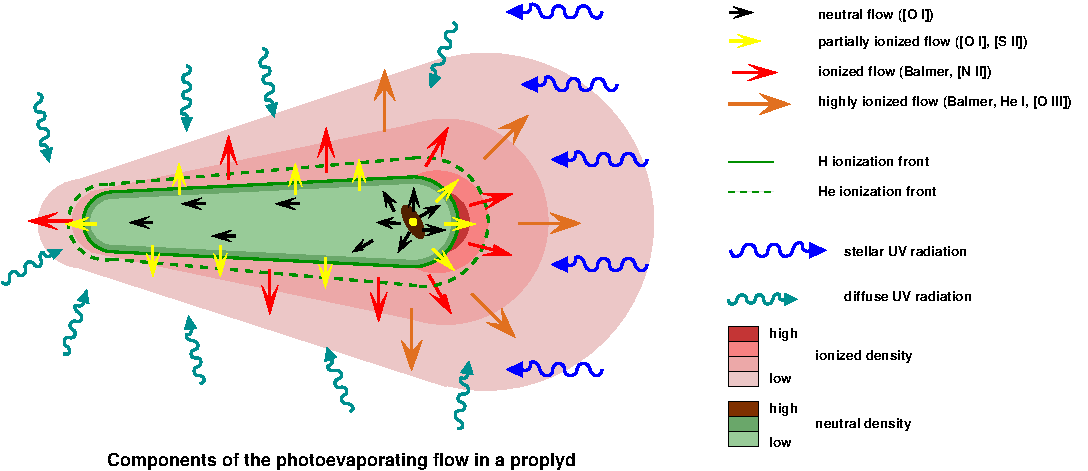
\includegraphics{modcart_col}}
\end{frame}

\begin{frame}
  \frametitle{Proplyds en la Nebulosa de Orión}
  \setkeys{Gin}{height=0.6\textheight}
  \includegraphics{OrionACS-CO-inset}\includegraphics{wind-geometry-compact}
\end{frame}

\begin{frame}
  \frametitle{Proplyds brillantes y oscuros}
  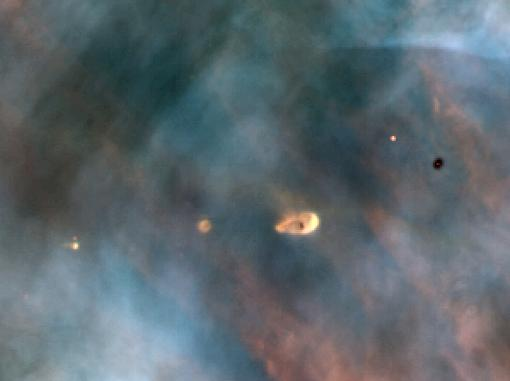
\includegraphics{HST10}
\end{frame}

\begin{frame}
  \frametitle{Orión en 3 dimensiones}
  \includemovie[label=orion-3d, autoplay, autopause, repeat, palindrome]
  {\textwidth}{0.75\textwidth}{hs-2001-13-a-high_quicktime.mov}
\end{frame}



\end{document}
